\chapter{序論}
\label{CBegin}

\section{研究背景}
\label{SBackground}

フォトリアルなコンピュータグラフィックス(Computer Graphics: CG)は、ハードウェアの発展や高性能コンピュータの普及により、近年ではさらに身近なものになっている。
%% 実物と見間違うほどのCGも珍しくなくなり、観客は実物とCGとの差異に敏感になってきている。
CG技術の発展により、コンピュータによって作成された画像に対して実写並みのリアリズムが要求されるようになってきた。
CGの歴史上においても、人間が現実世界で目にするものをそのままコンピュータ上に再現することが当初からの目標とされており、一部では実物とCGとの差異が埋まりつつあると言える。

CG技術においてリアリズムの追求はとどまるところを知らず、さらなる技術向上が目指されている。
また、現実世界にはCGによって十分に再現されていないさまざまな光学的な現象が依然として存在することも事実である。
そのため、多くの研究者たちがCGの表現力をさらに向上させるために研究・開発を行っている。

そうした中で、近年ではコンピュータ・ハードウェアの高速化により、リアルタイム(real-time:実時間)におけるCG映像の表現力が飛躍的に向上している。
リアルタイムで実写に迫る表現も可能になりつつあり\cite{jorge-jimenez2013}、今後もその要求は高まると考えられる。


\subsection{体積や厚みを考慮したコンピュータグラフィックス}
\label{SSVolumerendering}

CGは物体がどのように「見えるか」をコンピュータによって再現するために生み出された技術である。
そのため、「ものの見た目」においてもっとも重要である物体表面での光の反射のみを考慮するCGがある一方、臓器などの不透明な物体や煙や炎などといった粒子で満たされた一定の領域や体積を考慮しなくてはならない対象も存在する。
こうした対象を視覚化(visualize:ビジュアライズ)するためには、光が物体内部や粒子で満たされた領域内部を通過することによってその挙動にどのような影響が及ぼされるかについても考慮する必要がある。

たとえば、ボリュームレンダリング(Volume Rendering)の手法では、空間をボクセル(voxel)と呼ばれる六面体に分割し、遮る光の量を計算する。
ボクセルごとの密度も考慮しており、密度の大きなボクセルほど多くの光の量を遮る。
歴史的には、医療の分野で用いられるCT(Computed Tomography)データのビジュアライゼーションを目的とする視覚化手法の研究が重ねられていたが、1980年代にCGの分野でもボクセルを用いたボリュームデータの視覚化が行われるようになった\cite{cg-magic}。
ボリュームレンダリングは主に肉や骨、脂肪といった密度の違う領域をあわせ持つ人体の視覚化する方法として研究が始められたようである。

ほかには、パーティシペイティングメディア(participating media)という自然科学の分野における考え方を導入した手法がある。
煙や炎などは光が物体内部で吸収や散乱を起こしやすく、こうした光の吸収度や散乱度が非常に大きい領域はパーティシペイティングメディアと呼ばれる。
パーティシペイティングメディアをレンダリングするための技法はボリュームレンダリングの技法とともにボリュームをレンダリングするための技法として、CGの歴史上でほぼ同時期に登場した\cite{cg-magic}。

大理石や人体の皮膚といった半透明の材質をレンダリングするための技法として、サブサーフェイススキャッタリング(subsurface scattering)を考慮した手法も研究が盛んに行われている。
サブサーフェイススキャッタリングとは、一度物体内部に進入した光が物体内部で反射を繰り返し、光が入射した位置とは別の位置から外部へ向かって出射する光の挙動のことである。
自然界のほとんどの物体でこの現象が見られ、半透明の質感を持った大理石や皮膚などにおいて顕著に現れる。
サブサーフェイススキャッタリングを物理的に正確にレンダリングするためには非常に大きな計算不可がかかっていたものの、映画などでのフォトリアリスティックな表現への要求から研究が進み、現在ではすでに実時間での計算手法も開発されている\cite{garcia2012practical}。

以上のように、光が物体内部を通過するオブジェクトのレンダリングに関しては以前から研究が進んでおり成果を上げている。
しかし、いずれも全体の性質を代表して近似できる程度の微小な構造に対する光の挙動を再現したものであり、マイクロメートルオーダーの大きさの構造体が集合した物体に対する光の挙動までは扱っていない。

\subsection{生物発想のコンピュータグラフィックス}

皮膚や眼球など人間を対象としたCG表現に関してはこれまでに数多くの研究がなされているが\cite{jorge-jimenez2013}、人間以外にも動物や昆虫といったさまざまな生物のもつ光学現象を対象としたCG研究も近年では行われるようになってきている。
生物の発する体色などの色は発色のしくみが解明されていないものもあり、たとえば構造色といった表面微細構造によって色が変化するものも存在する。
構造色の定義は様々であるが、代表的な木下\cite{kinosita-木下修一2001総論}の定義によれば「光自体の性質が波長により異なることに由来した発色現像の総称」であり、通常の色素による発色と異なる。
そのため、角度や媒質などの観測条件によって色が変化するものが多い。
例えば、自然界ではコガネムシやモルフォチョウの翅などの昆虫の体色や孔雀の羽根などが該当する。
流体シミュレーションなどの現在盛んに行われている物理学をCGに応用した研究\cite{akinci2013versatile}と比較して、生物のモーションや体色などの生物学をCGに応用した研究はいまだ端緒についたばかりである。

%% \begin{figure}[hn]
%%   \centering
%%   
\includegraphics[width=3.0in]{./img/TEMP}
%%   \caption{構造色の例}
%%   \label{F}
%% \end{figure}

%% \subsection{リアルタイムでのハイクオリティレンダリング}

%% 近年ではコンピュータ・ハードウェアの高速化により、リアルタイム(real-time:実時間)におけるCG映像の表現力が飛躍的に向上している。
%% リアルタイムで実写に迫る表現も可能になりつつあり、今後もその要求は高まると考えられる。
%% \textcolor{red}{********}

\subsection{複眼と偽瞳孔}
\label{SSCompoundeyeandpseudopupil}

複雑な内部構造を有し、さらに生物に関連するものとして昆虫や甲殻類などの複眼が挙げられる。
複眼は個眼と呼ばれる小さな眼の集合体であり、それぞれの個眼にはレンズや色素細胞といったの光学現象に影響する部位が備わっている\figref{FYagi3LensPigment}。
複眼の見た目に関係する光学的な現象として偽瞳孔と呼ばれる現象がある。
偽瞳孔とは複眼表面に現れる黒い斑点模様\figref{FWhatIsPseudopupil}であり、個眼のレンズによる光の屈折作用と密接に関わっている。
\chapref{CKnowledge}で詳細を述べる。

\begin{figure}[htbp]
  \centering
  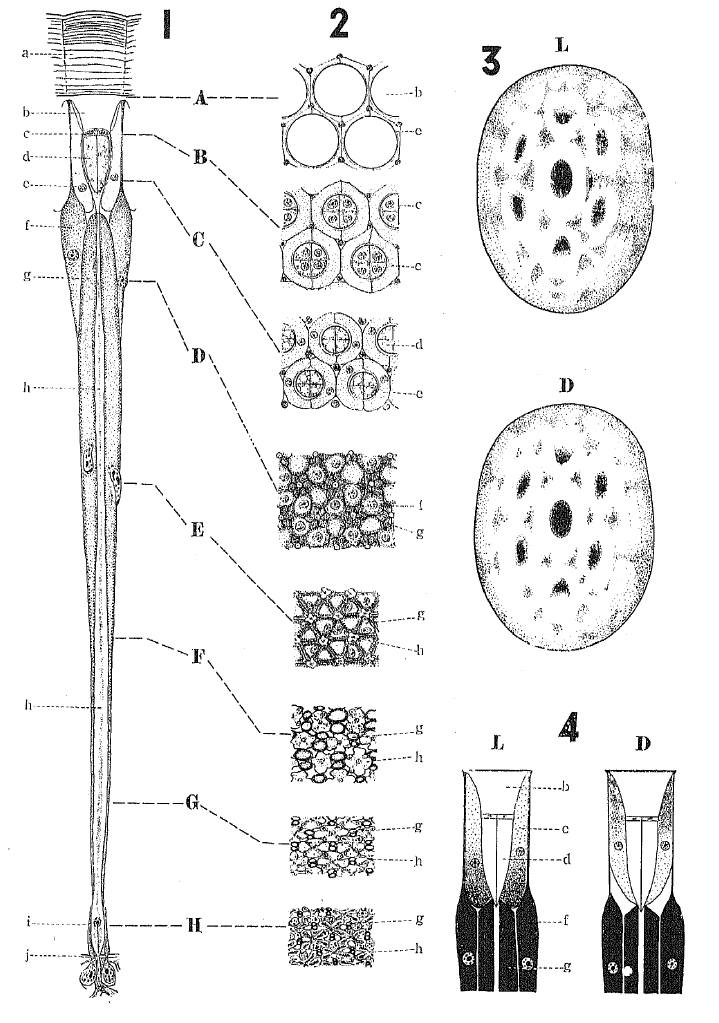
\includegraphics[width=3.0in]{./img/yagi3-lens-pigment.png}
  \caption{個眼の模式図(左)(\cite{yagi1955studies}より転載)}
  \label{FYagi3LensPigment}
\end{figure}

\begin{figure}[htbp]
  \centering
  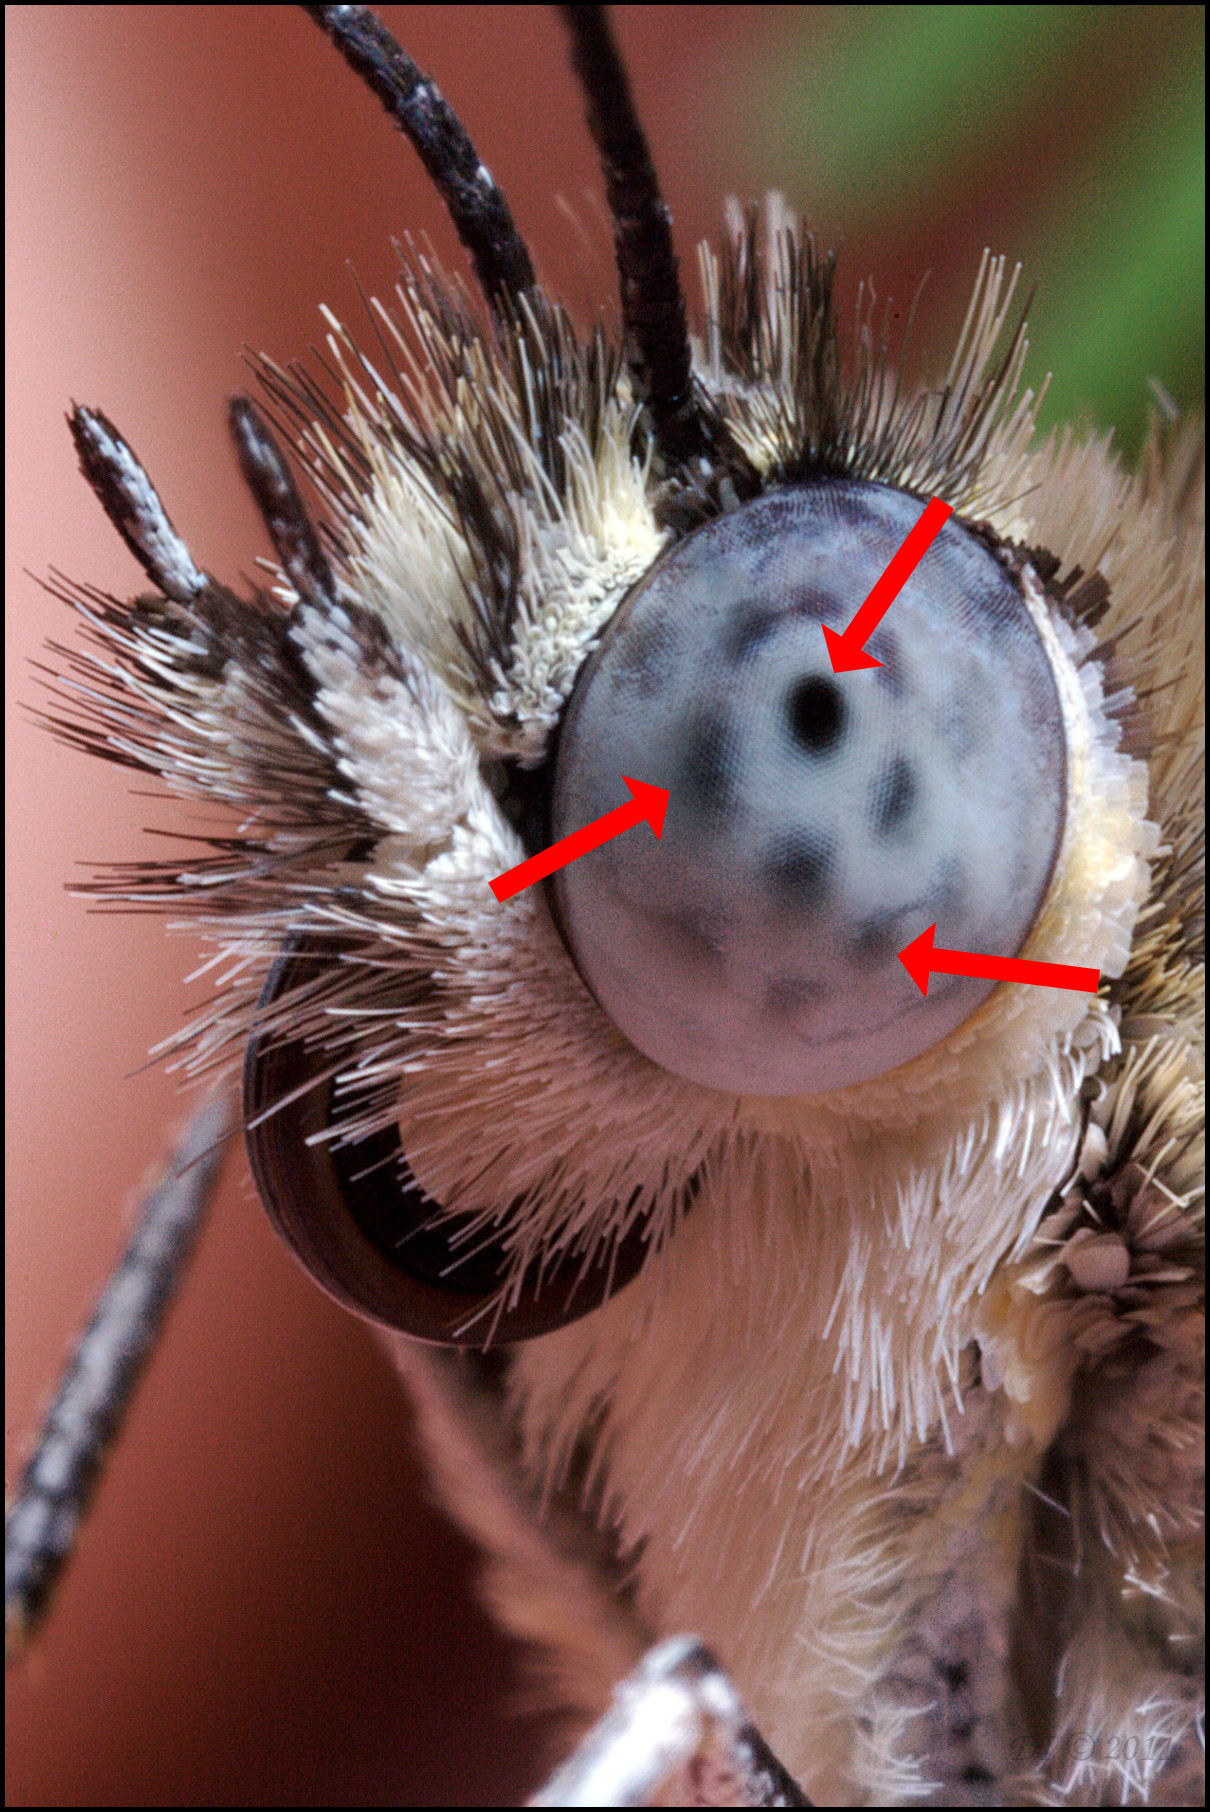
\includegraphics[width=3.0in]{./img/what_is_pseudopupil.png}
  \caption{偽瞳孔(\cite{flickr-blueeye}をもとに作成)}
  \label{FWhatIsPseudopupil}
\end{figure}


複眼を構成する個眼の数は非常に多く、さらに表面の構造が非常に複雑で細かいためコンピュータで精巧な形状を作成するのは現実的ではない。
また、精巧な形状のみを擬似的に表現する手法はCGにおいても研究が進んでおり、非常に高い効果を上げている。
例を挙げると、ディスプレイスメントマッピングやバンプマッピングなどの手法\cite{making-of-upside-down}では、ポリゴン表面に変位情報や法線情報を付加するによって複雑で細かい表面形状を少ない計算量で表現することを可能にしている\figref{FDisplacement}。
現在ではアートやエンターテイメントの分野において昆虫の複眼を表現する際にこれらの手法を利用するのが一般的となっている。
しかしながら、上記の手法では複眼の表面的な形状を再現するのみにとどまっており、複眼の内部構造を考慮した光学的現象を再現するまでには至っていない。
すなわち、先述の偽瞳孔をCGを用いて光学的に再現するための手法は未発展であると言える。

\begin{figure}[hn]
  \centering
  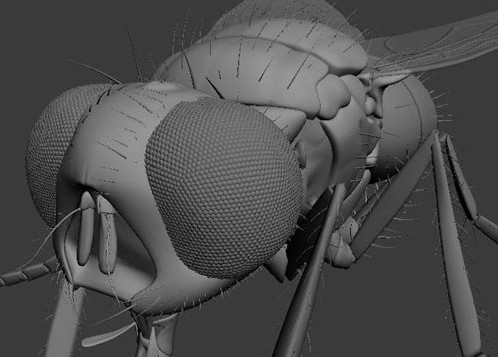
\includegraphics[width=3.0in]{./img/displacement.jpg}
  \caption{ディスプレイスメントマッピングによる複眼(\cite{making-of-upside-down}より転載)}
  \label{FDisplacement}
\end{figure}

%可能なら先生の画像を使わせてもらう


\section{本研究の目的}
\label{SObjective}

これまでに紹介したように、技術の進歩にともなって、コンピュータグラフィックスに対する要求は増してきつつある。
さらに、今後はリアルタイムレンダリングにおいても高精細で写実的な表現が求められると考えられる。
\secref{SSVolumerendering}で述べたように、物体内部を通過する光を考察したレンダリング(rendering)手法が生み出されてはいるものの、より複雑で光の挙動に影響を与えるような内部構造を持つ物体のレンダリングに関しては対象ごとに個別の手法を考案する必要がある。
本研究では、昆虫などの複眼表面に現れる光学現象として\secref{SSCompoundeyeandpseudopupil}で述べた偽瞳孔に着目し、この現象のCGによるリアルタイムでの表現手法の研究および開発を目的とする。

\section{本論文の構成}
\label{SPaper_structure}

本論文の構成について述べる。
次の\chapref{CRelatedWork}では、本研究と関連のある技術手法や生物分野で複眼について調査等を行った研究を紹介する。
\chapref{CKnowledge}では、周辺技術として本研究の基礎となるシェーダアルゴリズムについて解説を行う。
続いて\chapref{CExperiment}では、過去の研究を踏まえて本研究で実際に行った予備実験について説明する。
実験結果を踏まえて\chapref{CMethod}では、本研究で提案するシミュレーション手法を述べる。
最後に、応用事例として「かごしまアートフェスタ2014」にて行った展示について掲載する。
